% Propósito: mostrar que una función inversa recupera la variable de entrada.
% Origen: d(t)=ct y t(d)=d/c para c=4 m/s, t=3 s y d=12 m.
% Descripción accesible: un bloque de tiempo de 3 s se conecta con uno de
% distancia de 12 m mediante una flecha directa d=ct; una segunda flecha en
% sentido contrario, t=d/c, recupera el tiempo. En ambos casos c=4 m/s.
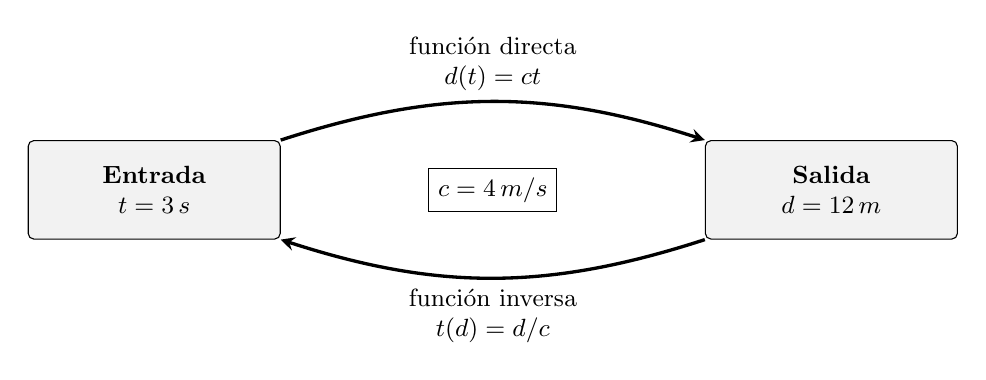
\begin{tikzpicture}[
    font=\small,
    >=stealth,
    valor/.style={
        draw,
        rounded corners=2pt,
        minimum width=3.2cm,
        minimum height=1.25cm,
        align=center,
        fill=black!5
    }
]
    \node[valor] (tiempo) at (0,0) {\textbf{Entrada}\\\(t=3\,\text{s}\)};
    \node[valor] (distancia) at (8.6,0) {\textbf{Salida}\\\(d=12\,\text{m}\)};

    \draw[->,very thick] (tiempo.north east) to[bend left=18]
        node[above,align=center]{función directa\\\(d(t)=ct\)}
        (distancia.north west);
    \draw[->,very thick] (distancia.south west) to[bend left=18]
        node[below,align=center]{función inversa\\\(t(d)=d/c\)}
        (tiempo.south east);

    \node[draw,align=center,fill=white] at (4.3,0)
        {\(c=4\,\text{m}/\text{s}\)};
\end{tikzpicture}
